\section{Verification Methodology}
\label{sec:verifier_method}

The verifier of record for the Truth Beam substrate is \emph{Phase~G}: a custom epsilon-prediction U-Net trained as a conditional density model over genuine $(C_t, E_t)$ capture--emission pairs and used as an anomaly scorer rather than a generator. We emphasise at the outset that Phase~G never denoises an image and never synthesises a capture. It is a diffusion model only in the sense that it learns to predict the noise that was added to a known-genuine capture under a forward process conditioned on the emission that was projected at that step; the magnitude of its noise-prediction residual $\lVert \hat{\epsilon}-\epsilon \rVert^2$ then serves as the verification score. This section details the network, its conditioning pathway, the training objective and corpus, the residual-energy scoring rule, and the architecture- and data-matched shuffled control that establishes the result is driven by genuine chain-coupling and not by generic emission statistics or an architectural artifact. The scope of every claim is the same-rig, two-session corpus (D2 and V10); we make no cross-rig, cross-camera, cross-projector, or cross-subject claim anywhere in this section.

\subsection{Network architecture}

The backbone is a custom epsilon-prediction U-Net, denoted \texttt{DiffusionDiagnosticUNet}, with \num{39770000} trained parameters (39.77M) at the canonical checkpoint (step \num{25000}). It is deliberately \emph{not} a diffusion transformer (DiT) and \emph{not} a Stable Diffusion model; it is a compact, purpose-built U-Net tailored to the packed colour-filter-array (CFA) representation of the raw capture. The network operates on a four-channel packed CFA input ($\text{in\_ch}=4$) and predicts a four-channel noise field $\hat{\epsilon}$ of matching shape ($\text{out}=4$).

The encoder/decoder has four down-sampling and four up-sampling scales built from residual blocks. The base channel width is $\text{base\_ch}=96$, and the channel multipliers $(1,2,4,4)$ give per-stage channel counts of $(96,192,384,384)$; the two deepest stages share a width of 384 channels. Self-attention is applied at the deepest scale only ($\text{attn\_at}=(\mathrm{False},\mathrm{False},\mathrm{False},\mathrm{True})$), which restricts the (quadratic) attention cost to the most coarsely sampled feature map while leaving the shallower, higher-resolution stages purely convolutional --- a standard cost--capacity trade-off for image-scale U-Nets.

Phase~G is evaluated full-frame at an operating resolution of $768\times1024$. The packed-CFA capture is cropped (region $y\in[0,1704]$, $x\in[155,2433]$ from the $(4,2300,2660)$ packed tensor) and resampled with area interpolation; the emission is resized from its native $(3,1080,1920)$ tile to the same grid. No tiling, patching, or temporal context is used: each $(C_t,E_t)$ pair is scored independently, frame by frame. We note the modest aspect-ratio adjustment this entails (cropped aspect $\approx 0.748$ resampled to $0.75$, a distortion of $\approx 0.3\%$); the shuffled control below shares this exact preprocessing, so any such artifact is differenced out of the headline comparison.

\subsection{ControlNet-style emission conditioning}

A central design decision is \emph{how} the emission $E_t$ enters the network. We do not concatenate $E_t$ to the camera input $C_t$. Instead, $E_t$ is conditioned in via a ControlNet-style hint pathway~\cite{zhang2023controlnet}. A dedicated \emph{HintEncoder} --- a four-stage strided $3\times3$ convolutional stack (stride 2 at each stage, $/16$ total down-sampling) with GroupNorm and GELU nonlinearities --- produces a multi-scale embedding of the emission hint. At each U-Net scale the encoded hint is injected by \emph{addition} into the down-path features through a per-scale zero-convolution adapter:
\[
\text{fused}_\ell \;=\; \text{down}_\ell(\text{prev}) \;+\; \text{adapter}_\ell\!\big(\text{HintEncoder}_\ell(E)\big),
\]
with one $1\times1$ zero-initialised convolution per scale (four adapters in total). Because the adapters are zero-initialised, the network's output at the start of training is exactly the unconditional model: the emission hint contributes nothing until training ramps it up, so any learned dependence on $E$ is acquired, not assumed. The hint input carries $\text{hint\_in\_ch}=11$ channels, a layout inherited from the F-A~v1 editor's hint encoder; the exact per-channel composition is an inherited implementation detail rather than a quantity we re-derive here.

To keep the conditional pathway honest, training applies classifier-free-guidance-style conditioning dropout: with probability $\text{cond\_drop\_prob}=0.2$, the emission hint is zeroed for a training example. This both regularises the conditioning and makes available, at evaluation time, a meaningful \emph{unconditional} reference (the same network with $E$ zeroed), against which the value of the genuine emission can be measured.

\subsection{Diffusion objective and forward process}

Conditioning aside, the training objective is standard epsilon-prediction. We adopt the denoising diffusion probabilistic model framework~\cite{ho2020ddpm} with the cosine noise schedule of Nichol \& Dhariwal~\cite{nicholdhariwal2021} (offset $s=0.008$) over $T=1000$ diffusion timesteps. The diffusion timestep $\tau$ is sampled uniformly from $\{1,\dots,1000\}$. To avoid clashing with the chain index $t$ of $C_t, E_t, S_t$, we write $x_0$ for the clean diffusion target (a genuine capture, $x_0 \equiv C_t$) and $x_\tau$ for its noised version. The forward (noising) process is the usual closed-form $q$-sample,
\[
x_\tau \;=\; \sqrt{\bar{\alpha}_\tau}\,x_0 \;+\; \sqrt{1-\bar{\alpha}_\tau}\;\epsilon,
\qquad \epsilon \sim \mathcal{N}(0,\mathbf{I}),
\]
with $\bar{\alpha}_\tau$ the cumulative product of the cosine schedule. The model is trained to predict the injected noise from the noised capture and the emission hint, under the simple mean-squared objective
\[
\mathcal{L} \;=\; \mathbb{E}_{\tau,\epsilon}\,\big\lVert \hat{\epsilon}(x_\tau, E, \tau) - \epsilon \big\rVert^2,
\]
with conditioning dropout applied as above. There is no perceptual term, no adversarial term, and no auxiliary classifier: the network learns only to model the noise residual of a genuine capture given its genuine emission.

\subsection{Training corpus and optimisation}

Phase~G is trained on real, same-rig capture--emission pairs drawn from two recording sessions: D2 (\num{5992} frames, recorded under the v9 chain) and V10 (\num{3743} frames, recorded under the v10 chain). Training therefore spans two chain protocols on the same rig, which underlies the same-rig cross-protocol observation discussed in \Cref{sec:results_main}; it is not a cross-rig statement. Held-out evaluation blocks are excised from training with a guard band: \num{1200} D2 frames and \num{500} V10 frames (\num{1700} total) are held out, a guard band of \num{60} frames brackets each held-out block, and the remaining training rows are stride-decimated (stride 3, $\approx\num{2478}$ training rows). The D2 held-out blocks are $(1298,1698)$, $(2796,3196)$, $(4294,4694)$ and the V10 blocks are $(1110,1360)$, $(2345,2595)$.

Optimisation runs for \num{25000} steps with AdamW~\cite{loshchilov2019adamw} at learning rate $10^{-4}$ on a cosine learning-rate schedule with a \num{500}-step linear warm-up, with batch size 2 per GPU across 8 GPUs (effective batch 16) under bf16 autocast. Training wall time is approximately \SI{17000}{\second} ($\approx 4.7$ hours) on $8\times$ A100. The epsilon-prediction MSE converges to $\approx 5\times10^{-4}$ (step-\num{25000} batch loss \num{0.000626}; per-batch loss is noisy at batch size 2). No validation-loss curve was logged during training, so model selection is on the final checkpoint; we note this as a limitation in the absence of an early-stopping diagnostic.

\subsection{Residual-energy scoring}

At inference Phase~G does not run the reverse diffusion process. The verification score for a candidate pair $(C,E)$ is the energy of the noise-prediction residual,
\[
\text{score}(C,E) \;=\; \big\lVert \hat{\epsilon} - \epsilon \big\rVert^2 ,
\]
evaluated under the model's own forward process. To make the score stable and timestep-aware we fix five evaluation timesteps spanning the schedule, $\mathrm{ALL\_TIMESTEPS}=(50,150,300,500,750)$, and average over $K_{\mathrm{NOISE}}=4$ independent noise draws per $(C,E,\tau)$. Each noise draw is seeded by the global frame index so the score is reproducible across evaluation shards. The total cost per scored pair is therefore $5\times4 = 20$ forward passes, with the per-pair MSE averaged over those passes. Benchmarked on an A100 in bf16, a single forward pass takes \SI{329}{\milli\second} (batch 1, $\tau=300$, mean of 20 reps), so a full $(C,E)$ score is $\approx\SI{6.6}{\second}$ at batch 1, or $\approx\SI{1.75}{\second}$ with the $K=4$ noise samples batched.

The interpretation is direct: a genuine pair, whose capture lies in the high-density region of the conditional model given its true emission, yields a small residual; a mispaired or substrate-altered pair yields a larger residual. Empirically the discriminative signal is strongest at small $\tau$ and decays as $\tau$ rises, consistent with the substrate signature residing in fine, low-noise structure: on the D2 held-out blocks the per-timestep wrong-versus-correct gap falls from $\Delta_{\text{wrong}}\approx\num{0.00594}$ at $\tau=150$ to $\approx\num{0.00339}$ at $\tau=300$ and $\approx\num{0.00165}$ at $\tau=500$, while per-timestep separability remains saturated (AUROC~$=1.000$) at every reported timestep. \Cref{fig:zhist,fig:ecdf} present the distributional form of this score across the corpus, and \Cref{fig:atypicality} shows its spatial footprint.

\begin{figure}[t]\centering
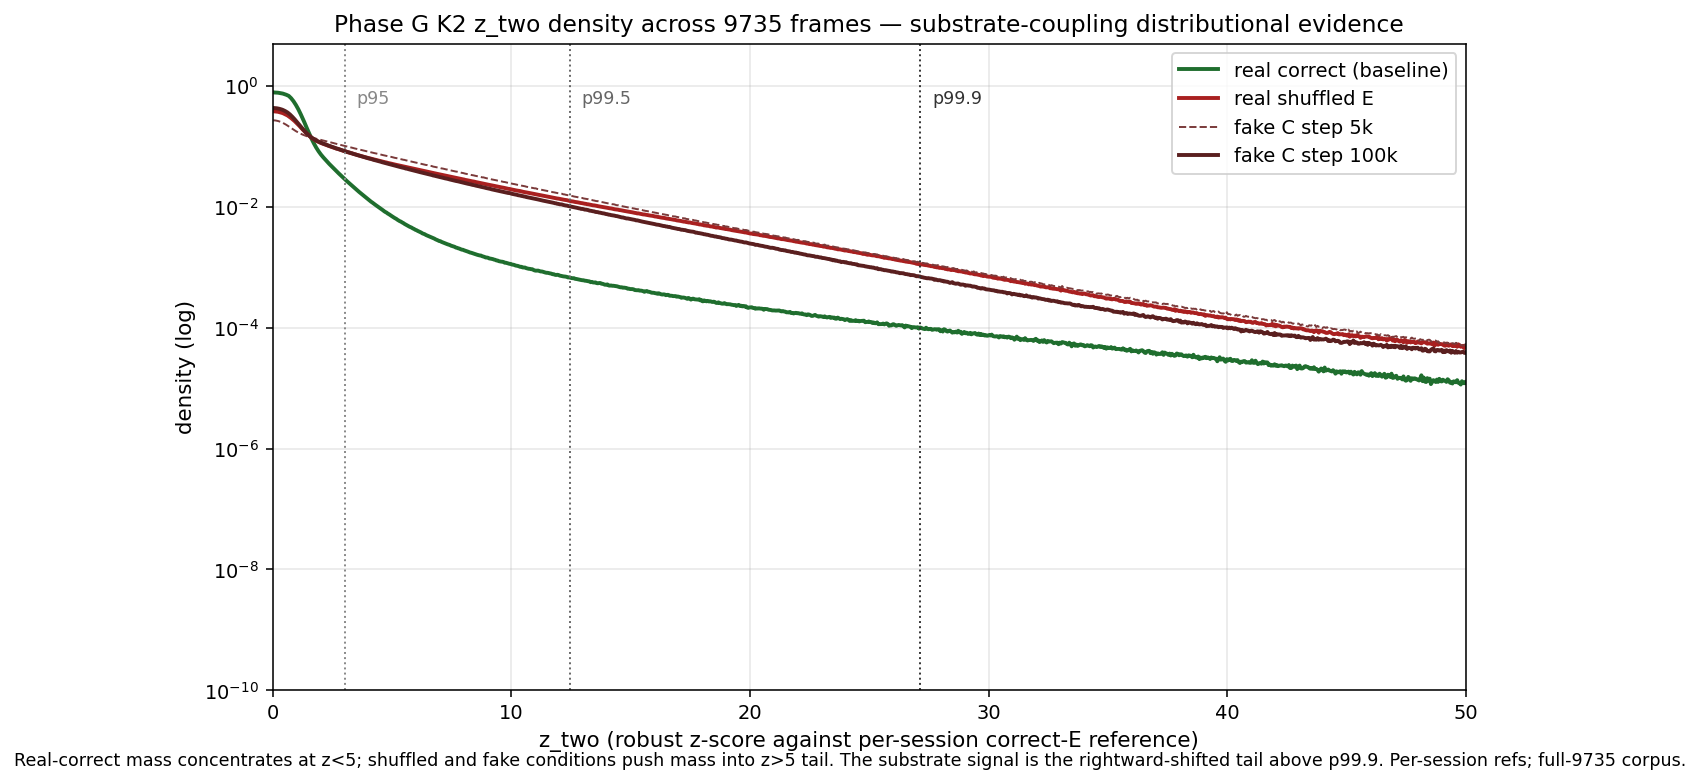
\includegraphics[width=\linewidth]{figures/fig_zhist.png}
\caption{Distributional evidence for chain-coupling. Per-pixel $z_{\text{two}}$ log-density across \num{9735} frames for four conditions: real-correct (baseline), real-shuffled $E$, synthetic $C$ at training step 5k, and step 100k. Real-correct mass concentrates at $z<5$; shuffled and synthetic conditions carry heavy right tails. The discriminative substrate signal is the rightward-shifted tail above the p99.9 percentile. $z_{\text{two}}$ is a robust $z$-score against the per-session correct-$E$ reference; percentile markers (p95, p99.5, p99.9) are drawn from the full-\num{9735} corpus.}
\label{fig:zhist}
\end{figure}

\begin{figure}[t]\centering
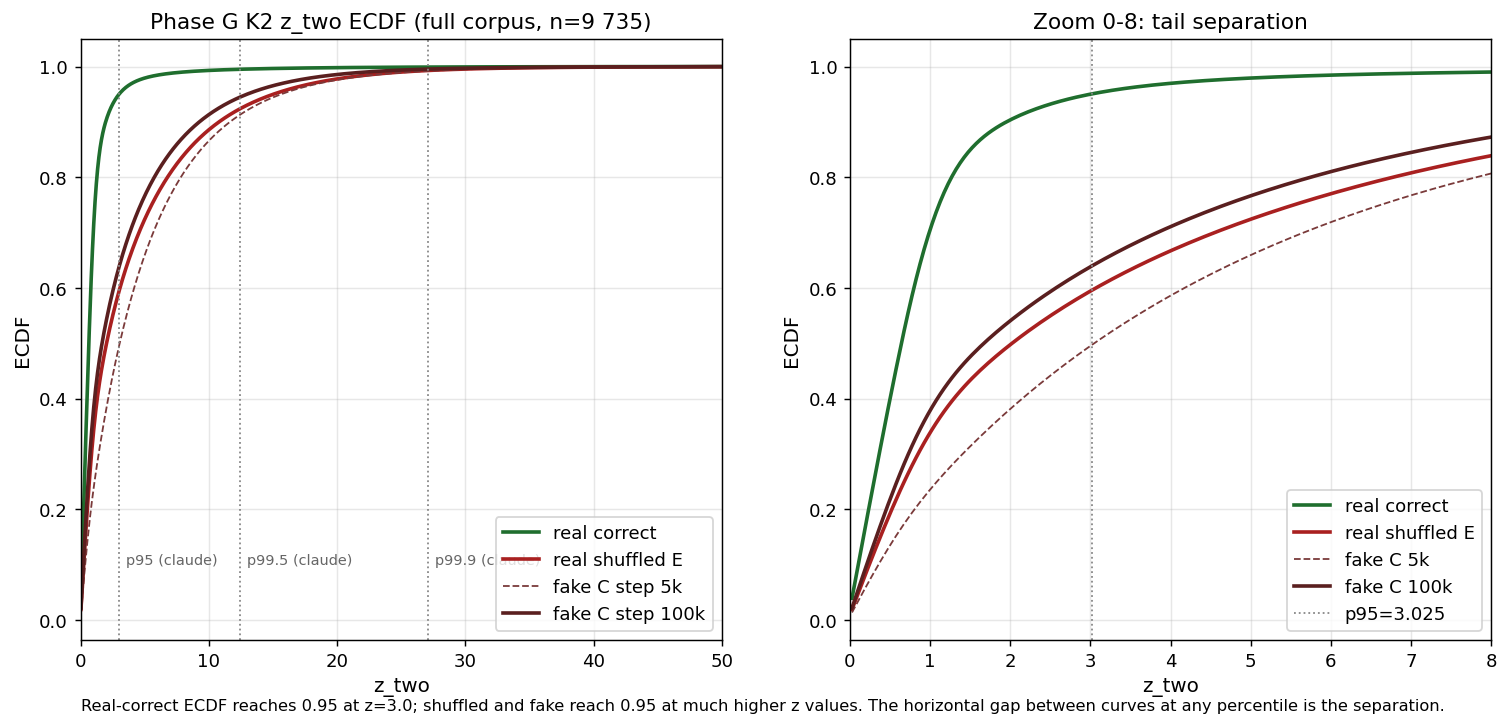
\includegraphics[width=\linewidth]{figures/fig_ecdf.png}
\caption{Empirical CDF of $z_{\text{two}}$ (full corpus, $n=\num{9735}$). Left: full range; right: zoom to $z\in[0,8]$ showing tail separation. The real-correct ECDF reaches $0.95$ at $z=3.0$, while shuffled and synthetic conditions reach $0.95$ only at substantially higher $z$. The horizontal gap between curves at any percentile is the per-pixel separation margin. Per-session reference; percentile markers from the full-\num{9735} corpus.}
\label{fig:ecdf}
\end{figure}

\subsection{The shuffled-E control}

A near-perfect verifier raises an immediate question: is the network truly detecting the physical coupling between a capture and \emph{its own} emission, or is it merely exploiting generic statistics of the emission images, or an artifact of the architecture and training recipe? To answer this we train a second model that is \emph{identical in every respect} --- same \texttt{DiffusionDiagnosticUNet} architecture, same \num{39770000} parameters, same hint pathway and zero-conv adapters, same cosine schedule, same $T=1000$, same corpus, same optimiser, same step budget, same held-out blocks, and the identical $768\times1024$ preprocessing --- with exactly one difference: the genuine pairing between capture and emission is destroyed by \emph{shuffling}. The shuffled model is trained to predict the noise of capture $C_t$ conditioned on a mismatched emission. If the main model's discrimination came from generic emission statistics or from the network/recipe rather than from genuine chain-coupling, the shuffled model would inherit it; if it came from the physical coupling, the shuffled model has nothing to learn and must sit at chance.

The shuffled control sits at chance. Its correct-versus-wrong separability is $\mathrm{AUROC}\approx 0.5006$ (D2 $0.5006377$, V10 $0.500625$), and its mean residual gap between correct and wrong emissions is $\Delta_{\text{wrong}}\approx 10^{-7}$ (D2 $6.98\times10^{-8}$ with 95\% CI $[3.89,\,11.8]\times10^{-8}$; V10 $1.39\times10^{-7}$). By contrast the main model achieves $\mathrm{AUROC}=1.000$ with $\Delta_{\text{wrong}}\approx 4\times10^{-3}$ --- roughly five orders of magnitude larger. The shuffled control's $\Delta_{\text{wrong}}$ confidence interval technically excludes zero, but the effect is so many orders of magnitude smaller than the main model's that it is operationally indistinguishable from chance. This control is the load-bearing falsification test: because it differs from the main model only in the real-versus-shuffled pairing, it isolates the contribution of genuine chain-coupling and rules out generic emission statistics and an architecture/recipe artifact as the source of the separation. It does not by itself exclude every conceivable shortcut --- confounds that survive identical preprocessing, such as session-level idiosyncrasies, are addressed separately by the cross-session ablation of \Cref{sec:results_main_generalization}.

It is important to keep the shuffled control distinct from the offset-based ``wrong-$E$'' used in the headline AUROC. The headline correct-versus-wrong AUROC pairs a genuine capture against \emph{temporally mispaired real emissions} (frame offsets $\{-2,+2,-15,+15,+30\}$ and the lag sweep); the shuffled control instead retrains the entire model under a destroyed pairing. The two are complementary: the offset evaluation shows the main model resolves the correct emission against close temporal neighbours, while the shuffled control shows the capability itself is not an artifact. A separate synthetic-positive control (an isotropic photometric injection, $\mathrm{blur}(E)$ added to $C$) confirms the scoring pipeline can detect an $E$-dependent signal it is meant to detect ($\mathrm{AUROC}=1.000$, $\Delta_{\text{wrong}}\approx 1.1$--$1.2\times10^{-3}$); we caution, per its own design, that an isotropic photometric injection may have different spectral structure from a real chain signal, so it corroborates the pipeline rather than the main result.

\subsection{Unconditional reference and multi-method cross-checks}

The conditioning-dropout design also yields an \emph{unconditional} reference (the trained main model evaluated with $E$ zeroed). Comparing a genuine pair against this reference measures how much the true emission lowers the residual relative to having no emission at all; the resulting correct-versus-unconditional AUROC is $0.977$ (D2) and $0.942$ (V10). This is necessarily a softer contrast than correct-versus-wrong, because the zeroed-$E$ input is itself somewhat out of distribution; we report it as supporting evidence for emission-dependence, not as the headline.

Finally, we cross-check the Phase~G verdict against additional methods on genuine captures (\Cref{fig:multimethod}). Phase~G and a binder-residual method are treated as verifier-tier; autoencoder taps (AE-64f, AE-DGW) are shown for cross-checking only and are explicitly labelled \textsc{diagnostic}, because they exhibit weak coupling-specificity and are not relied upon as verifiers. On genuine frames all four methods agree on a typical (low-residual) verdict, but only the verifier-tier methods carry quantitative weight in this report.

\begin{figure}[t]\centering
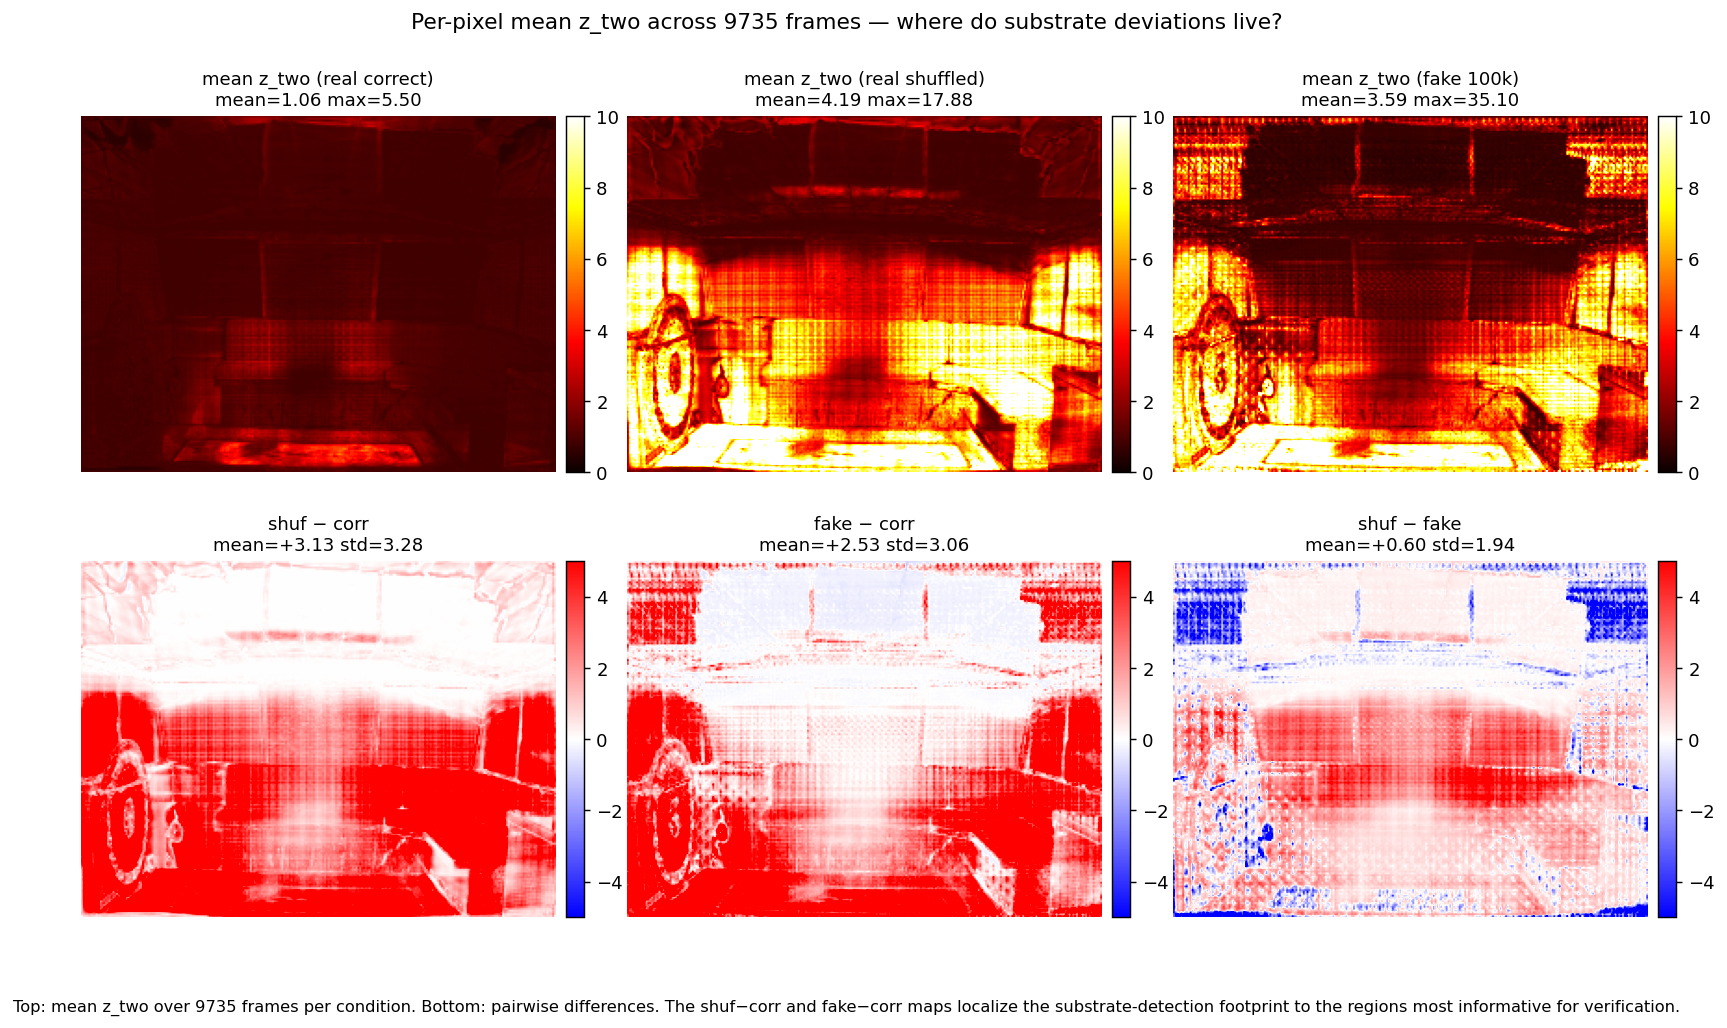
\includegraphics[width=\linewidth]{figures/fig_atypicality.png}
\caption{Spatial footprint of the substrate signature. Top: per-pixel mean $z_{\text{two}}$ across \num{9735} frames for real-correct (mean $1.06$), real-shuffled ($4.19$), and synthetic-100k ($3.59$) conditions. Bottom: pairwise differences (shuffled $-$ correct, synthetic $-$ correct, shuffled $-$ synthetic). The shuffled-minus-correct and synthetic-minus-correct maps localise the substrate-detection footprint to the frame regions most informative for verification, concentrated away from the central subject. Computed over the full \num{9735}-frame corpus with per-session references; no per-frame normalization.}
\label{fig:atypicality}
\end{figure}

\begin{figure}[t]\centering
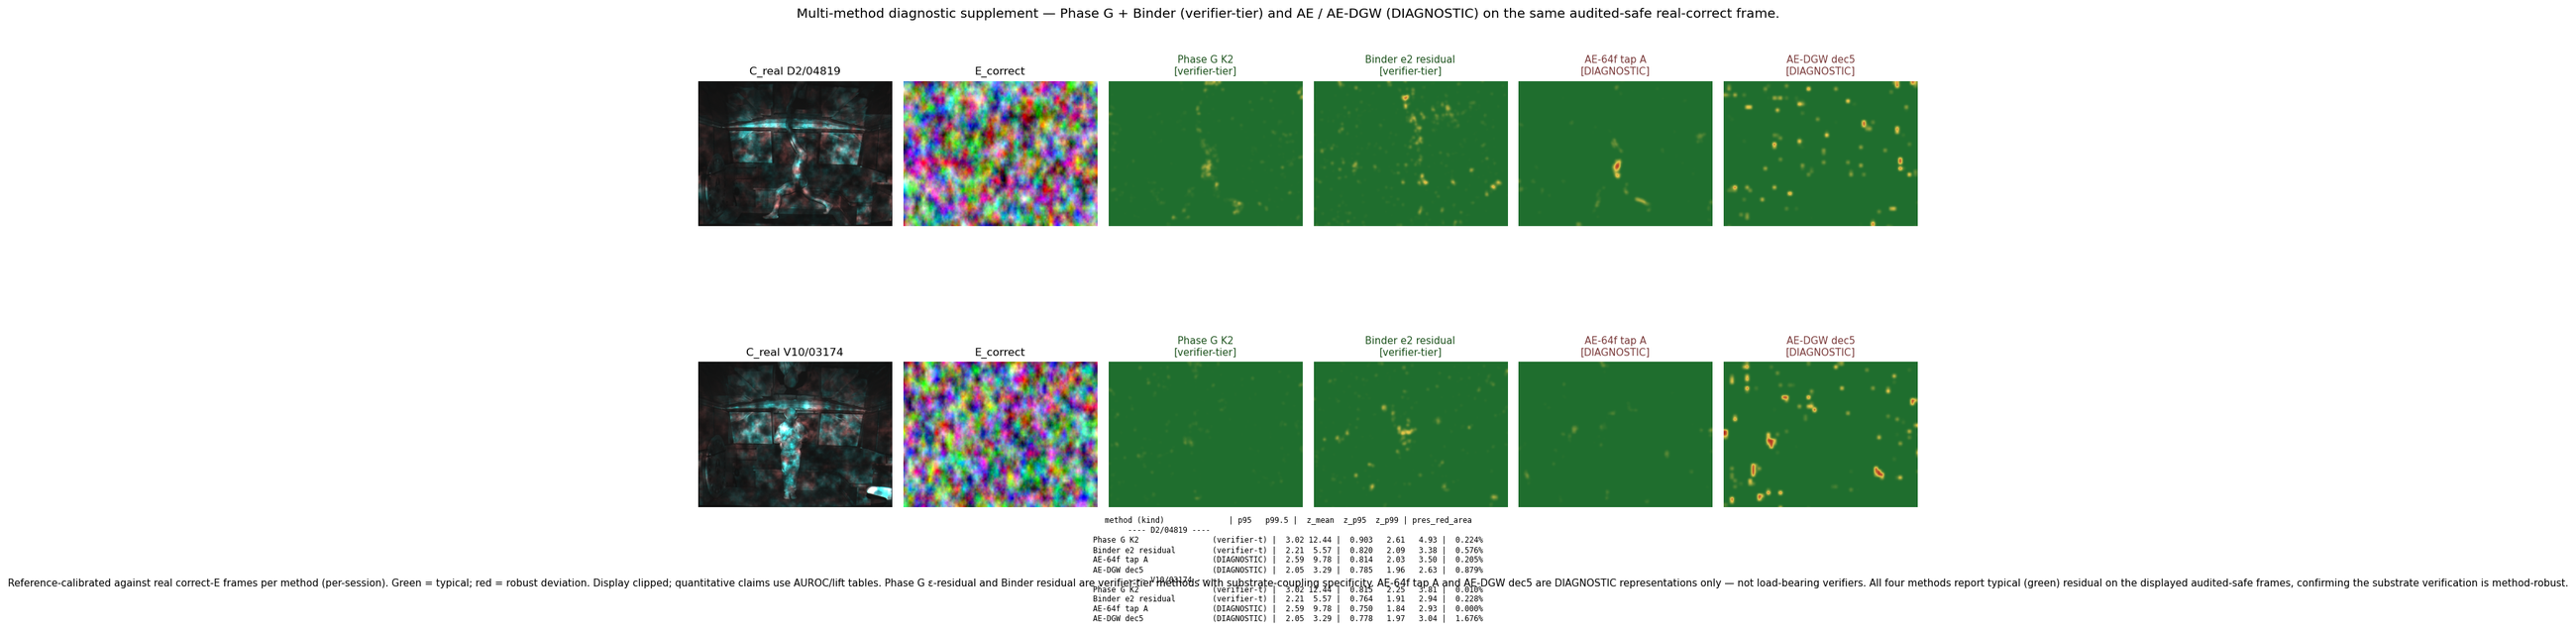
\includegraphics[width=\linewidth]{figures/fig_multimethod.png}
\caption{Multi-method agreement on genuine captures. Two audited-safe real-correct frames (D2 row 4819, V10 row 3174) scored by four methods: Phase~G K2 and Binder e2 (verifier-tier) and AE-64f tap A and AE-DGW dec5 (labelled \textsc{diagnostic}, not verifier-tier). All four report typical (green) residual on these genuine frames. Each method uses its own per-session reference with common thresholds within the panel; display is clipped; quantitative claims rest on the results reported in the text, not on this display. The AE methods are shown for cross-checking only and are not used as verifiers because they exhibit weak coupling-specificity.}
\label{fig:multimethod}
\end{figure}

\subsection{Scope and limitations of the methodology}

Two methodological scope guards apply throughout. First, the held-out evaluation blocks are drawn from the same two sessions used for training, so the $\mathrm{AUROC}=1.000$ result measures \emph{within-session} (same-rig) generalisation; cross-session generalisation is established separately by the single-session ablations of \Cref{sec:results_main_generalization}, and nothing in this work establishes cross-rig, cross-camera, cross-projector, or cross-subject generalisation. Second, the scoring rule is deliberately a residual-\emph{energy} statistic ($\epsilon$-MSE), which (as developed in later sections) is dominated by high-frequency structure; alternative scoring functions reweight which regions of the residual field carry the signal, and the choice of $\epsilon$-MSE is a design decision rather than a unique optimum. The methodology described here is what the remaining results sections evaluate; robustness against a trained, adaptive forger (the stronger F-A~v2 attacker, which is in design only and not trained) is out of scope for this methodology and is treated strictly as future work.
